\begin{question}{}{}
Montrer que dans un graphe, il existe toujours au moins deux sommets de même degré.
\end{question}

\begin{myproof}
Soit $G = (S,A)$ un graphe.
On note $n = \mathrm{car d}(S)$ à l'ordre de $G$.

On sait que  $\forall s \in S, \; \mathrm{deg} (S) \in \{0, 1, 2, \ldots, n-1\}$

Il y a deux cas :
\begin{enumerate}
    \item $\exists s \in S$, $\mathrm{deg} (s) = n-1$, alors $G$ ne peut pas avoir de sommet isolé.
        Donc, $\forall s\in S$, $\mathrm{deg} (S) \in \{1, 2,\ldots, n-2,n-1\}$, donc il existe au moins 2 sommets de même degré d'après le principe des tiroirs. (range $n$ objets dans $p$ tiroirs avec $p<n$, alors il existe au moins un tiroir contenant au moins 2 objets)
    \item $G$ a de sommet isolé. Même façon.
\end{enumerate}
\end{myproof}

\begin{question}{}{}
Un graphe $G = (S, A)$ est dit biparti si son ensemble de sommets peut-être partitionné en deux sous-ensembles $S_1$ et $S_2$ tels que chaque arête ait une extrémité dans $S_1$ et l’autre dans $S_2$.

1. Montrer que si $G = (S, A)$ est biparti alors $\mathrm{card} (A) \le  \mathrm{card}(S)^{2}/4$.

2. Montrer que si $G = (S, A)$ est biparti alors $\exists s \in S, \;\mathrm{ deg}(s) \le  \mathrm{card} (S)/2$. 

3. Un graphe biparti est-il nécessairement connexe ? Et acyclique ?

4. Un graphe biparti peut-il contenir un cycle de longueur impair ?
\end{question}

\begin{myproof}
\begin{enumerate}
    \item Soit $G = (S,A)$ un graphe biparti.

        On note $n = \mathrm{car d}(S)$, $k = \mathrm{car d} (S_1)$ donc $\mathrm{car d} (S_2) = n-k$.

        $\forall s \in S_1$, $\mathrm{deg} (s) \le n-k$, donc $\mathrm{car d} (A) \le k(n-k)$

        On étuidie la fonction $f: k \mapsto k(n-k) = nk -k^{2}$, c'est un polynôme de degré 2 qui admet un maximum en $x = n / 2$ qui vaut  $f(n / 2) = n^{2} / 4$.

    \item Soit $G= (S,A)$ un graphe biparti. On note $n = \mathrm{car d} (S)$. Par l'absurde, on suppose que $\forall s \in S, \; \mathrm{deg} (s) > n / 2$.

        Sachant que $2 \mathrm{card} A = \sum_{s \in S} \mathrm{deg} (s) > \sum _{s \in S} n/2 = \frac{n^{2}}{4} $

        Donc $\mathrm{car d} (A) > n^{2} / 4$ ce qui est absurde.
    \item Non, non
    \item Non
\end{enumerate}

\end{myproof}

\begin{question}{Graphe de Kneser}{}
  Soient $n$ et $k$ deux entiers tels que $1 \le k < n$, Le \textbf{graphe de Kneser} est le graphe dont les sommets correspondent aux parties à $k$ éléments d'un ensemble à $n$ éléments, et deux sommets sont relié si et seulement s'ils correspondent à des parties disjoints.
\begin{enumerate}
  \item Détermine l'ordre et la taille de $K _{n,k}$
\end{enumerate}
\begin{figure}[H] %h:当前位置, t:顶部, b:底部, p:浮动页
    \centering
    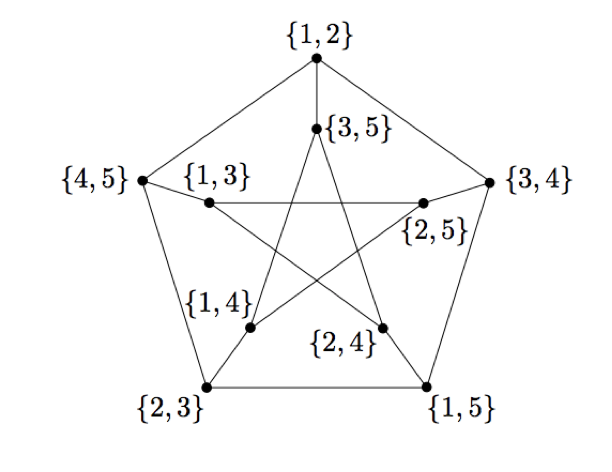
\includegraphics[width=0.4\textwidth]{./assets/Kneser Graph.png}
    \caption{Kneser Graph}
    \label{fig:Kneser-Graph}
\end{figure}


\end{question}

\begin{myproof}{}{}
\begin{enumerate}
  \item $S _{n,k}$ est l'ensemble des parties à $k$ éléments de $E$. 
    \[
      S _{n,k} = \{ e \subset E, \; \mathrm{card}(e) = k\} \implies \mathrm{card}(S _{n,k}) = \binom{n}{k}
    \]
\end{enumerate}
\end{myproof}


